\documentclass{beamer}
%\documentclass[xcolor={dvipsnames,table}]{beamer}
%\usetheme{Warsaw}
%\usetheme{AnnArbor}
%\usetheme{Frankfurt}
\usetheme{Madrid}
%\setbeamertemplate{title page}[default][colsep=-0bp,rounded=false]
%\setbeamertemplate{frametitle}[default][colsep=-4bp,rounded=false,shadow=false]
%\setbeamertemplate{blocks}[rounded][shadow=false]


\title{PSET5: Ordered Collections \\ Priority Queues}


\date{March 17, 2023}

\author{Anusha Murali}


\usepackage{tikz-qtree}
\begin{document}

%\frame{\titlepage}

\begin{frame}[fragile]
\titlepage

\end{frame}


\begin{frame}[fragile]
\frametitle{Tasks to do}

\begin{block}{Part II: Implement Ordered Collections with Priority Queues}
\begin{enumerate}
\item Complete \textcolor{red}{ListQueue}: elements are stored a list
\item Complete \textcolor{red}{TreeQueue}: elements are stored in a BST
\item Complete \textcolor{red}{BinaryHeap}: elements are stored in a balanced binary tree
\end{enumerate}
\end{block}
\end{frame}


\begin{frame}[fragile]

\vspace*{0.5in}

\centerline{\huge TreeQueue}

\vspace*{0.2in}
\begin{center}
Task: Use a BST to implement the signature of PRIOQUEUE .
\end{center}

\end{frame}





%%%%%%%%%%%%%%%%%%%%%%%
\begin{frame}[fragile]
\frametitle{Step 1 Load Files}

\begin{block}{Load Files}
\begin{enumerate}
\item \# \#use "order.ml"
\item \# \#use "orderedcoll.ml"
\item \# \#use "prioqueue.ml"
\end{enumerate}
\end{block}
\end{frame}


\begin{frame}{fragile}
\frametitle{Step 2: Complete the {\tt TreeQueue} functor}


\begin{block}{Complete the types}
\hspace*{1.0in}type elt = Elt.t \\
\hspace*{1.0in}type queue = T.collection
\end{block}

\begin{block}{Complete empty}
\hspace*{1.0in}let empty = T.empty
\end{block}

\begin{block}{Complete is\_empty}
\hspace*{1.0in}let is\_empty (q : queue) = (q = T.empty)
\end{block}

\begin{block}{Complete add}
\hspace*{1.0in}let add (e : elt) (q : queue) = T.insert e q
\end{block}

\end{frame}




\begin{frame}{fragile}
\frametitle{Step 2: Complete the {\tt TreeQueue} functor}

\begin{block}{Complete take}
\hspace*{1.0in}let take (q : queue) =\\
\hspace*{1.15in}      let highest\_pri = T.getmin q in \\
\hspace*{1.15in}      (highest\_pri, (T.delete highest\_pri q))
\end{block}

\begin{block}{Complete to\_string}
\hspace*{1.0in}let to\_string (q: queue) : string = \\
\hspace*{1.15in}      T.to\_string q
\end{block}

\end{frame}


\begin{frame}{fragile}
\frametitle{Step 2: Complete the {\tt ListQueue} functor}

\begin{block}{Re-load prioqueue.ml (with your completed functions)}
\begin{enumerate}
\item \# \#use "prioqueue.ml"
\end{enumerate}
\end{block}

\begin{example}
Now the examples in the next slides should work
\end{example}
\end{frame}
      

\begin{frame}{fragile}
\frametitle{Test all the new functions}

\begin{block}{First create the \textcolor{yellow}{IntTreeQueue} module}

\vspace*{0.1in}

\noindent
        \# {\bf module IntTreeQueue = (TreeQueue(IntCompare) : \\
 \hspace*{0.5in}  PRIOQUEUE with type elt = IntCompare.t);;}

\end{block}

\end{frame}


\begin{frame}{fragile}
\frametitle{Test add function}

\begin{example}
\begin{enumerate}
\item First create an empty TreeQueue called myQ \\
        \# {\bf  let myQ = IntTreeQueue.empty;;}
\item Insert 65\\
 \# {\bf let myQ = IntTreeQueue.add 65 myQ};;
\end{enumerate}
\end{example}

\tikzset{every tree node/.style={minimum width=2.5em,draw,circle},
         blank/.style={draw=none},
         edge from parent/.style=
         {draw,edge from parent path={(\tikzparentnode) -- (\tikzchildnode)}},
         level distance=1.5cm, sibling distance=1.5cm}
\begin{center}
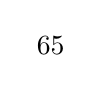
\begin{tikzpicture}
 \Tree [.65  ]
 \end{tikzpicture}
\end{center}

\begin{example}
Print the queue:\\

\# {\bf IntTreeQueue.to\_string myQ;;} \\

\hspace*{1in} \textcolor{red}{Output:} - : string = "Branch (Leaf, [65], Leaf)"

\end{example}

\end{frame}


\begin{frame}{fragile}
\frametitle{Test add function}

\begin{example}
\begin{enumerate}
\item Now insert 40\\
 \# {\bf let myQ = IntTreeQueue.add 40 myQ};;
\end{enumerate}
\end{example}

\tikzset{every tree node/.style={minimum width=2.5em,draw,circle},
         blank/.style={draw=none},
         edge from parent/.style=
         {draw,edge from parent path={(\tikzparentnode) -- (\tikzchildnode)}},
         level distance=1.5cm, sibling distance=1.5cm}
\begin{center}
\begin{tikzpicture}
 \Tree [.65  [.40 ]  \edge[blank]; \node[blank]{};   ]
\end{tikzpicture}
\end{center}


\begin{example}
Print the queue:\\

\# {\bf IntTreeQueue.to\_string myQ;;} \\

\hspace*{0.2in} \textcolor{red}{Output:} - : string = "Branch (Branch (Leaf, [40], Leaf), [65], Leaf)"

\end{example}

\end{frame}


\begin{frame}{fragile}
\frametitle{Test add function}

\begin{example}
\begin{enumerate}
\item Now insert 50\\
 \# {\bf let myQ = IntTreeQueue.add 50 myQ};;
\end{enumerate}
\end{example}

\tikzset{every tree node/.style={minimum width=2.5em,draw,circle},
         blank/.style={draw=none},
         edge from parent/.style=
         {draw,edge from parent path={(\tikzparentnode) -- (\tikzchildnode)}},
         level distance=1.5cm, sibling distance=1.5cm}
\begin{center}
\begin{tikzpicture}
 \Tree [.65  [.40  \edge[blank]; \node[blank]{}; [.50 ] ]  \edge[blank]; \node[blank]{};   ]
\end{tikzpicture}
\end{center}

\end{frame}



\begin{frame}{fragile}
\frametitle{Test add function}

\begin{example}
\begin{enumerate}
\item Now insert 70\\
 \# {\bf let myQ = IntTreeQueue.add 70 myQ};;
\end{enumerate}
\end{example}

\tikzset{every tree node/.style={minimum width=2.5em,draw,circle},
         blank/.style={draw=none},
         edge from parent/.style=
         {draw,edge from parent path={(\tikzparentnode) -- (\tikzchildnode)}},
         level distance=1.5cm, sibling distance=1.5cm}
\begin{center}
\begin{tikzpicture}
 \Tree [.65  [.40  \edge[blank]; \node[blank]{}; [.50 ]  ]  [.70 ] ]
\end{tikzpicture}
\end{center}

\end{frame}




\begin{frame}{fragile}
\frametitle{Test add function}

\begin{example}
\begin{enumerate}
\item Now insert 30\\
 \# {\bf let myQ = IntTreeQueue.add 30 myQ};;
\end{enumerate}
\end{example}

\tikzset{every tree node/.style={minimum width=2.5em,draw,circle},
         blank/.style={draw=none},
         edge from parent/.style=
         {draw,edge from parent path={(\tikzparentnode) -- (\tikzchildnode)}},
         level distance=1.5cm, sibling distance=1.5cm}
\begin{center}
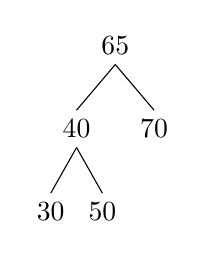
\begin{tikzpicture}
 \Tree [.65  [.40  [.30 ]  [.50 ]  ]  [.70 ] ]
\end{tikzpicture}
\end{center}

\end{frame}


\begin{frame}{fragile}
\frametitle{Test add function}

\tikzset{every tree node/.style={minimum width=2.5em,draw,circle},
         blank/.style={draw=none},
         edge from parent/.style=
         {draw,edge from parent path={(\tikzparentnode) -- (\tikzchildnode)}},
         level distance=1.5cm, sibling distance=1.5cm}
\begin{center}
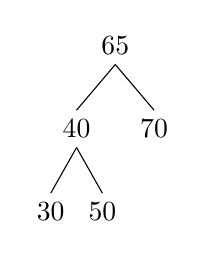
\begin{tikzpicture}
 \Tree [.65  [.40  [.30 ]  [.50 ]  ]  [.70 ] ]
\end{tikzpicture}
\end{center}

\begin{block}{Print myQ using the provided "to\_string" function}
{\bf \# IntTreeQueue.to\_string myQ;;}

\vspace*{0.1in}
"Branch (Branch (Branch (Leaf, [30], Leaf), [40], Branch (Leaf, [50], \\ \hspace*{1.95in}Leaf)), [65], Branch (Leaf, [70], Leaf))"
\end{block}

\end{frame}


%%%%%%%%%%%%%%%

\begin{frame}{fragile}
\frametitle{Test take function}

\begin{example}
\begin{enumerate}
\item The take function returns the element with the highest priority (i.e: smallest value) and the remaining queue\\
 \# {\bf let (hiPri, myQ) = IntTreeQueue.take myQ};;
\item The value of {\bf hiPri = 30} and the new {\bf myQ} is shown below
\end{enumerate}
\end{example}

\tikzset{every tree node/.style={minimum width=2.5em,draw,circle},
         blank/.style={draw=none},
         edge from parent/.style=
         {draw,edge from parent path={(\tikzparentnode) -- (\tikzchildnode)}},
         level distance=1.5cm, sibling distance=1.5cm}
\begin{center}
\begin{tikzpicture}
 \Tree [.65  [.40  \edge[blank]; \node[blank]{};   [.50 ]  ]  [.70 ] ]
\end{tikzpicture}
\end{center}

\end{frame}







\begin{frame}{fragile}
\frametitle{Important comments on TreeQueue}
\begin{block}{Average and worst-case time complexity}
\begin{enumerate}
\item On the average, the BST is nearly balanced. So, the height of the tree is $\log n$. Hence the  average time complexity to search an element is $O(\log n)$
\item In the worst case, the elements are inserted in sorted order. This will result in a completely right-skewed or left-skewed tree. So, the worst-case time complexity to search an element is $O(n)$
\end{enumerate}
\end{block}

\end{frame}


\end{document}

